%% This is an example first chapter.  You should put chapter/appendix that you
%% write into a separate file, and add a line \include{yourfilename} to
%% main.tex, where `yourfilename.tex' is the name of the chapter/appendix file.
%% You can process specific files by typing their names in at the 
%% \files=
%% prompt when you run the file main.tex through LaTeX.

\begingroup%
\makeatletter%
\cleardoublepage%
\let\newpage\relax%
\let\clearpage\relax%
\vspace*{\fill}%
\vspace*{\dimexpr-50\p@-\baselineskip}% Remove the initial
%% -default- 50pt gap (plus 1 line) 
\chapter[LOBSTAHS: An Adduct-Based Lipidomics Strategy for Discovery and Identification of Oxidative Stress Biomarkers]{LOBSTAHS: An Adduct-\\Based Lipidomics Strategy for Discovery and \\Identification of Oxidative Stress Biomarkers}
\label{chap3}
\let\thefootnote\relax\footnote{{\setlength{\parindent}{0pt}Reproduced with permission from:\\\\Collins, J. R., B. R. Edwards, Helen F. Fredricks, and B. A. S. Van Mooy. 2016. LOBSTAHS: An adduct-based lipidomics strategy for discovery and identification of oxidative stress biomarkers. \emph{Analytical Chemistry} \emph{88}:7154-7162; doi:\href{http://dx.doi.org/10.1021/acs.analchem.6b01260}{10.1021/acs.analchem.6b01260}\\\\\copyright 2016 American Chemical Society}}
\vspace*{\fill}%
\endgroup%

\clearpage
\section{Abstract}
Discovery and identification of molecular biomarkers in large LC/MS datasets requires significant automation without loss of accuracy in the compound screening and annotation process. Here we describe a lipidomics workflow and open-source software package for high-throughput annotation and putative identification of lipid, oxidized lipid, and oxylipin biomarkers in high-mass-accuracy HPLC-MS data. Lipid and Oxylipin Biomarker Screening through Adduct Hierarchy Sequences, or LOBSTAHS, uses orthogonal screening criteria based on adduct ion formation patterns and other properties to identify thousands of compounds while providing the user with a confidence score for each assignment. Assignments are made from one of two customizable databases; the default databases contain 14,068 unique entries. To demonstrate the software's functionality, we screened more than 340,000 mass spectral features from an experiment in which hydrogen peroxide was used to induce oxidative stress in the marine diatom \emph{Phaeodactylum tricornutum}. LOBSTAHS putatively identified 1,969 unique parent compounds in 21,869 features that survived the multi-stage screening process. While \emph{P. tricornutum} maintained more than 92\% of its core lipidome under oxidative stress, patterns in biomarker distribution and abundance indicated remodeling was both subtle and pervasive. Treatment with 150 $\mu$M H\textsubscript{2}O\textsubscript{2} promoted statistically significant carbon-chain elongation across lipid classes, with the strongest elongation accompanying oxidation in moieties of monogalactosyldiacylglycerol, a lipid typically localized to the chloroplast. Oxidative stress also induced a pronounced reallocation of lipidome peak area to triacylglycerols. LOBSTAHS can be used with environmental or experimental data from a variety of systems and is freely available at \url{https://github.com/vanmooylipidomics/LOBSTAHS}.
\clearpage
\section{Introduction}
Reactive oxygen species (ROS) represent a persistent source of stress in virtually all biological systems (Apel and Hirt, 2004; Crastes de Paulet et al., 1988). The negative cellular effects of ROS include protein damage, mutation of DNA, and lipid peroxidation (Lesser, 2006). While the profound effects of oxidative stress have been documented extensively in the lipids of mammals (Kuhn and Borngraber, 1999; Strassburg et al., 2012; Wenk, 2010), ROS can induce equally significant and wide-ranging remodeling of cell lipidomes in terrestrial and marine plants (Andreou et al., 2009; Buseman et al., 2006; Vu et al., 2012). These ROS can act through a variety of enzymatic and abiotic mechanisms to produce a broad and heterogeneous suite of lipid products whose bioactivity and diversity make them ideal as molecular biomarkers. These products include both oxidized intact polar lipids (ox-IPL; e.g., oxidized phospholipids; Vu et al., 2012) as well as oxylipins, the smaller, direct derivatives of fatty acids. Lipid biomarkers (both oxidized and unoxidized) can be used to characterize the effects of ROS in humans from cancer (Thomas et al., 2013) and other diseases such as atherosclerosis (Haller et al., 2014); in the marine environment, lipids can be used to diagnose various sources of biological and abiotic stress, including those imposed by nutrient limitation (Carini et al., 2015; Van Mooy et al., 2009) and viral infection (Fulton et al., 2014; Vardi et al., 2009). The potency and specificity that make lipids useful as biomarkers of oxidative stress also support their function as bioactive ``infochemicals'' (Ianora and Miralto, 2010; Pohnert, 2008; Vardi, 2008). In the ocean, for example, oxylipins have been shown to regulate different interspecific interactions among marine microbiota (Balestra et al., 2011; Casotti et al., 2005; Miralto et al., 1999; Ribalet et al., 2008) and the metabolism of sinking marine particles by heterotrophic bacteria (Edwards et al., 2015).

For several reasons, there exist few comprehensive methods to screen, identify, and annotate large numbers of these oxylipins and oxidized lipids alongside the many unoxidized lipids from which they can originate (Strassburg et al., 2012; Wenk, 2010). Oxylipins, like their parent lipids, have a wide diversity of structures and biochemical functions (Br\"{u}gger, 2014; Hol\v{c}apek, 2015; Strassburg et al., 2012). They can be produced enzymatically (Andreou et al., 2009; Andreou and Feussner, 2009; Lamari et al., 2013) or abiotically (Girotti, 1998; Triantaphylides et al., 2008), often occurring in very low abundance relative to their intact polar lipid (IPL) precursors (Sparvero et al., 2010; Wenk, 2010). Finally, unique and tailored computational strategies are required to analyze the large volumes of data necessary for comprehensive lipidomics or metabolomics (Hol\v{c}apek, 2015; Spickett and Pitt, 2015).

The limited number of analytical strategies developed specifically to assess the effects of oxidative stress on the lipidomes of humans (Strassburg et al., 2012) and mammals (Balvers et al., 2012; Bruins et al., 2013) have generally focused on traditional oxylipins, such as hydroperoxy, hydroxy, epoxy, oxo, and ketol fatty acids, while ignoring most molecular precursors and intermediates. For example, direct-infusion mass spectrometry has been used to identify select oxylipins simultaneously with their unoxidized IPL and ox-IPL precursors in the model plant \emph{Arabidopsis thaliana}, but these studies used manual data analysis methods to examine oxidation of compounds containing only C\textsubscript{16} and C\textsubscript{18} fatty acids (Buseman et al., 2006; Vu et al., 2012). Ni et al. (2015) employed a shotgun approach to identify oxidized lipids in rat cardiomyocytes, but their analysis was limited only to intact carbonylated phospholipids. The commercial LipidSearch software (Thermo Scientific) can identify some oxidized lipids using MS/MS fragmentation spectra, but this capability does not extend to oxylipins derived from fatty acids.

We developed a new, rules-based screening approach that can be used to identify a broad range of IPL, nonpolar lipids, ox-IPL, and oxylipins in large, high-mass-accuracy HPLC-ESI-MS datasets. Lipid and Oxylipin Biomarker Screening through Adduct Hierarchy Sequences, or LOBSTAHS, is implemented as an open-source package for R (R Core Team, 2015) and integrates with the existing packages xcms (Benton et al., 2010; Smith et al., 2006; Tautenhahn et al., 2008) and CAMERA (Kuhl et al., 2012). The software is centered around a novel screening methodology that exploits the unique tendency of lipids to form adduct ions in consistent, diagnostic patterns of abundance that remain relatively consistent across sample types (e.g., for phosphatidylcholine in positive ion mode, {[}M+H{]}\textsuperscript{+} \textgreater{} {[}M+Na{]}\textsuperscript{+} \textgreater{} {[}M+NH\textsubscript{4}+ACN{]}\textsuperscript{+} \textgreater{} {[}M+2Na-H{]}\textsuperscript{+} \textgreater{} {[}M+K{]}\textsuperscript{+}). Using lipid data from cultures of a mutant strain of a marine diatom designed for studies of oxidative stress (van Creveld et al., 2015), we demonstrate how LOBSTAHS can be used to resolve conflicting compound assignments, examine differential expression of compounds across experimental treatments, discover and identify potential ox-IPL and oxylipin biomarkers, and identify potential isomers and isobars.

LOBSTAHS annotates each compound assignment with a confidence score, allowing the user to define subsets for further analysis. While we apply LOBSTAHS here to identify potential biomarkers in a marine microorganism, it can be applied to any HPLC-ESI-MS dataset where the user expects the relative proportions of the various adduct ions of each analyte to remain constant across samples. LOBSTAHS requires data from a mass spectrometer having both high resolving power and high mass accuracy. While we developed the software using data acquired on a Thermo Exactive Plus Orbitrap instrument, LOBSTAHS could be used to analyze data acquired via FT-ICR-MS or, when sufficient allowances are made for mass resolution, a Q-TOF instrument.

\section{Theory and Design of Software and Databases}

\subsection{Databases}

\subsubsection{Design and Scope of Lipid-Oxylipin Databases}

LOBSTAHS draws compound assignments from customizable onboard databases that contain structural and adduct ion abundance data for various IPL, nonpolar lipids, ox-IPL, and oxylipins (\autoref{table:adn1}; \autoref{table:adn3}). Each database entry represents a different adduct ion of a potential analyte; because analytes present differently in positive and negative ionization modes, separate databases must be generated for compound identification in each mode. The standard package installation includes two default databases that contain entries for 14,068 unique compounds, some of them particular to marine algae (\autoref{table:adn1}; \autoref{table:adn3}). Alternatively, LOBSTAHS allows the user to generate his or her own databases; instructions are provided in the package documentation. The use of onboard databases distinguishes LOBSTAHS from other software packages that rely exclusively on external databases.

\subsubsection{Database Generation}

Databases are created in LOBSTAHS by pairing empirical data with an \emph{in silico} simulation. To generate the default databases, we first calculated exact masses for various triacylglycerols (TAG), free fatty acids (FFA), polyunsaturated aldehydes (PUA), and molecules belonging to eight different classes of intact polar diacylglycerol (IP-DAG). Within each of these classes, we calculated the masses of a wide range of possible structures having fatty acid (FA) moieties of different acyl chain length, unsaturation, and oxidation (\autoref{table:adn1}). While the default databases include entries for IPL and ox-IPL that contain primarily medium- and long-chain fatty acids, users may generate additional databases with entries for IPL composed of fatty acids of any length. The databases also include exact masses for several photosynthetic pigments common to the marine environment (\autoref{table:adn1}; \autoref{table:adn3}). TAG and IP-DAG are identified by the ``sum composition'' (Husen et al., 2013) of double bonds and acyl carbon atoms in each compound (e.g., PC 34:1, rather than PC 16:0-18:1).

\subsubsection{Determination of Relative Abundances of Adduct Ions for Inclusion in Databases}

During database generation, LOBSTAHS uses empirical data for the LC/MS adduct ion(s) typically formed by each compound's parent lipid class (\autoref{table:adn2}) to create several entries for each compound. Each of the entries represents a different adduct ion of its parent; the relative ranks of the adducts form the basis for the hierarchy-based screening of compound assignments at the core of our method. Relative adduct ion abundance data were gathered from previous work (Popendorf et al., 2013) and analysis of compounds commonly observed in cultures and environmental samples from marine microorganisms. Where possible, we confirmed the results using authentic standards for representative compounds. For ox-IPL, we applied adduct hierarchies observed for the corresponding, unoxidized IPL. We assumed ox-IPL would be unlikely to take charge on their oxidized functional group(s) during ionization, thus forming adducts similar to those of the corresponding unoxidized molecule. We confirmed this similarity in ionization behavior through manual inspection of several samples. Long-chain ox-IPL standards other than those containing aldehyde moieties are not available commercially.

A series of simple tables can be used to define additional analytes and/or adducts beyond those which are included in the default databases. For each new lipid or lipid class, LOBSTAHS requires (1) the elemental composition of the new lipid or parent moiety of the new lipid class, (2) a tabulation of expected adducts (defining, as necessary, any new adducts), (3) empirical adduct hierarchy data for any new adducts, and (4) if applicable, the ranges of acyl carbon atoms, double bonds, and oxidization states for which entries are to be generated. Specific instructions are contained in the online documentation for the software.

\subsection{Data Analysis Workflow}

\subsubsection{Lipidomics Workflow Based on xcms, CAMERA, and LOBSTAHS}

Because high resolving power and high mass accuracy are often not alone sufficient to resolve isobaric ions, or to distinguish among species that have identical monoisotopic masses but different elemental compositions (Kind and Fiehn, 2006), we employ high-performance liquid chromatography (HPLC) in lieu of a simple direct-infusion approach. Data must first be converted to an open-source format (.mzXML) and, if necessary, from profile to centroid mode. If data are acquired using ion mode switching, LOBSTAHS requires that positive and negative ion mode scan data also be extracted into separate files. Procedural details and an R script that can be used to automate these steps for data obtained from an Orbitrap instrument are described in the Supporting Information. For purposes of the present study, we consider two ions to be isobaric when the underlying features have different exact masses but the \emph{m/z} difference is less than the instrument's demonstrated mass accuracy (in this case, 2.5 ppm). Once data files have been converted and extracted, the existing R packages xcms (Benton et al., 2010; Smith et al., 2006; Tautenhahn et al., 2008) and CAMERA (Kuhl et al., 2012) are used for feature detection, peak grouping, chromatographic alignment, identification of pseudospectra, and discovery of features representing possible secondary isotope peaks (\autoref{fig:c3n1}, ``Pre-processing \& feature detection'').

\subsubsection{Database Assignments and Progressive Screening in LOBSTAHS using Orthogonal Criteria}

After pre-processing, screening and annotation are performed according to the workflow in \autoref{fig:c3n1}. First, initial compound assignments are applied to features from the database using a narrow \emph{m/z} mass tolerance specified by the user in ppm. A series of optional orthogonal screening criteria can then be applied to the features and their assignments. First, users may exclude from the dataset any features representing secondary isotope peaks; the presence of these features can be a significant obstacle in metabolomics (Clasquin et al., 2012; Ejsing et al., 2006; Layre et al., 2011). We programmed LOBSTAHS to exclude these secondary peaks, rather than merge the elements of each feature's isotopic envelope into a single parameter (Layre et al., 2011).

\begin{figure}[!p]
\centering
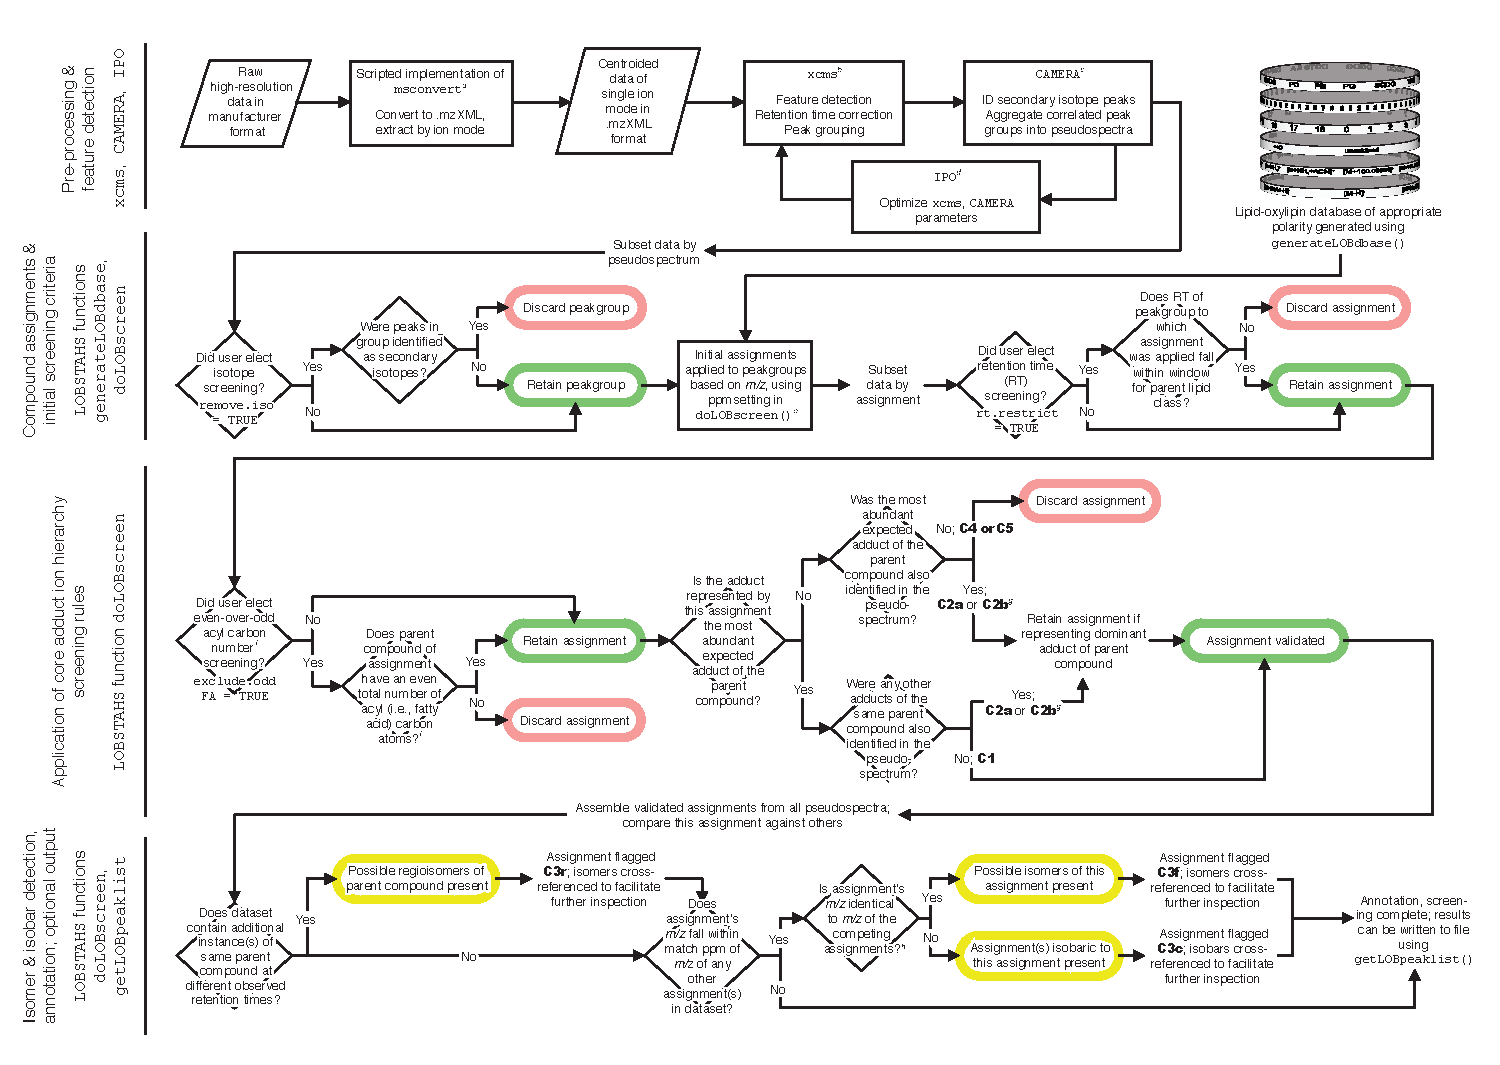
\includegraphics[width=1.05\textwidth]{Fig_3-1.pdf}
\captionsetup{font={footnotesize}}
\caption[Preparation, Screening, and Annotation of HPLC-MS Lipid Data Using LOBSTAHS]{Preparation, Screening, and Annotation of HPLC-MS Lipid Data Using LOBSTAHS. Annotation codes (in bold) may be applied as indicated; these are designed to assist the user in evaluating assignment confidence during subsequent data analysis.\\
\emph{\textsuperscript{a}} We automate several functions of the ProteoWizard msConvert tool (Kessner et al., 2008).\\
\textsuperscript{\emph{b},\emph{c}} xcms (Benton et al., 2010; Smith et al., 2006; Tautenhahn et al., 2008) was chosen for its command-line features and because it permits follow-on use of the R package CAMERA (Kuhl et al., 2012) to identify isotopes.\\
\emph{\textsuperscript{d}} IPO (Libiseller et al., 2015) can be used to optimize the values of parameters for some xcms and CAMERA functions.\\
\emph{\textsuperscript{e}} Multiple assignments will likely exist for many peakgroups in a typical dataset.\\
\emph{\textsuperscript{f}} This criterion may be useful when the subject dataset contains lipids of exclusively eukaryotic origin.\\
\emph{\textsuperscript{g}} In case C2a, the adduct ion hierarchy for the parent compound is completely satisfied; i.e., the pseudospectrum contains peakgroups representing every adduct ion of the compound of greater theoretical abundance than the least abundant adduct ion present. In case C2b, the adduct ion of greatest theoretical abundance and some lesser adduct ion is present, but adduct ions of intermediate abundance are not observed.\\
\textsuperscript{\emph{h}} Both outcomes may apply simultaneously at this decision point if the dataset contains isobars and isomers of the assignment.}
\label{fig:c3n1}
\end{figure}

Next, LOBSTAHS can screen the feature's retention time against a retention time ``window'' defined for the accompanying assignment's parent lipid class. LOBSTAHS includes a set of default retention time window data (\autoref{table:adn4}) for the chromatographic conditions we describe here. Detailed instructions for application of retention time data from other chromatographic methods are included in the Supporting Information. A third filter can then be applied to exclude assignments of IPL, ox-IPL, FFA, and PUA that contain an odd total number of acyl carbon atoms. We envision that this filter would be applied to data of exclusively eukaryotic origin: Since non-acetogenic fatty acid synthesis is confined almost exclusively to bacteria and archaea (Pearson, 2014), FA synthesized by eukaryotes will be composed of an even total number of carbon atoms.

After applying these initial optional criteria, LOBSTAHS then screens each assignment using adduct ion hierarchy data (\autoref{fig:c3n1}, ``Application of core adduct ion hierarchy screening rules''; \autoref{table:adn2}). This screening serves as the primary orthogonal filter to eliminate any confounding secondary isotopes and unassigned lipid-extractable features still remaining in the dataset. During this process, LOBSTAHS uses a series of rules to compare the relative abundance ranks of sets of adduct ion assignments that have the same parent compound. The package makes several annotations using simple codes that indicate the degree to which the assignment complies with the hierarchy rules (\autoref{fig:c3n1}, in bold). Assignments that fail the adduct ion hierarchy screening criteria are excised from the dataset and all remaining assignments in the dataset are then pooled.

Additional rules-based screening is then performed on the pooled data to identify and annotate possible isomers and isobars (\autoref{fig:c3n1}, ``Isomer \& isobar detection, annotation''). Codes can be applied to identify positional or regioisomers (code C3r), functional structural isomers (code C3f), or isobars (code C3c). LOBSTAHS can apply several of these different codes to a given assignment as long as the criterion for each is satisfied. Upon completion of screening, LOBSTAHS produces an R object containing the annotated dataset. Statistical analysis can then be performed in R on the final matrix of compound assignments, or the results can be exported to a .csv file for external analysis.

\section{Experimental Section}

\subsection{Model Dataset Used to Demonstrate the Workflow}

To demonstrate LOBSTAHS, we applied the workflow in \autoref{fig:c3n1} to examine the effect of oxidative stress on a model algal lipidome. For the analysis, we used lipid data collected from cultures of a mutant strain of the marine diatom \emph{Phaeodactylum tricornutum}, which was designed for studies of oxidative stress. In the study (van Creveld et al., 2015), a strain of \emph{P. tricornutum} (CCMP2561; Provasoli-Guillard National Center for Marine Algae and Microbiota) was genetically modified (Rosenwasser et al., 2014) to express a reduction-oxidation sensitive green fluorescent protein (roGFP) at different locations within the cell (Dooley et al., 2004; Hanson et al., 2004). Cultures of the transformants were treated with three concentrations of H\textsubscript{2}O\textsubscript{2} (0, 30, and 150 $\mu$mol L\textsuperscript{-1}) to evaluate the effects of peroxidation; culture conditions are described in van Creveld et al. (2015).

\subsection{Sample Collection and Extraction}

In the experiment, duplicate samples for lipid analysis were collected from each treatment at 4, 8, and 24 h timepoints. Two procedural blanks were also collected. Sample material was collected by vacuum onto 0.7 $\mu$m pore size glass fiber filters (GF/F), which were snap frozen in liquid nitrogen and then stored at -80$^{\circ}$C until thawed for extraction. Extraction was performed using a modified Bligh and Dyer (Bligh and Dyer, 1959) method described in Popendorf et al. (2013); an internal standard (dinitrophenyl-phosphatidylethanolamine, DNP-PE) and a synthetic antioxidant (butylated hydroxytoluene, BHT) were added at time of extraction. Lipid extracts were transferred to 2 mL HPLC vials, topped with argon, and stored at -80$^{\circ}$C prior to analysis. All chemicals used in sample extraction and chromatography were LC/MS grade or higher. Where used, water was obtained from a Milli-Q system without further treatment (EMD Millipore, Billerica, MA, USA).

\subsection{HPLC-ESI-MS Analysis}

Samples from the \emph{P. tricornutum} dataset were analyzed by HPLC-ESI-MS using a modification of the method described in Hummel et al. (2011) Lipid extracts were evaporated to near dryness and reconstituted in a similar volume of 7:3 acetonitrile:isopropanol. Headspace was filled with argon to minimize further oxidation. For HPLC analysis, an Agilent 1200 system (Agilent, Santa Clara, CA, USA) comprising temperature-controlled autosampler (4$^{\circ}$C), binary pump, and diode array detector, was coupled to a Thermo Exactive Plus Orbitrap mass spectrometer (ThermoFisher Scientific, Waltham, MA, USA). Chromatographic conditions, electrospray ionization source settings, MS acquisition settings, and procedures used for calibration of the mass spectrometer are described in the Supporting Information. Using authentic standards and two independent methods for MS feature detection, we determined the average relative mass uncertainty of the Exactive was \textless{} 0.2 ppm (\autoref{table:c3n1}; \autoref{table:adn6}); evaluation of these standards is discussed below.

\subsection{Analysis of \emph{P. tricornutum} Data Using LOBSTAHS}

xcms, CAMERA, and LOBSTAHS were then used to identify and annotate lipidome components in the positive ionization mode data. The R package IPO (Libiseller et al., 2015) was used to optimize settings for several xcms functions, and a 2.5 ppm mass uncertainty tolerance was used to obtain database matches in LOBSTAHS. Using the annotated output we obtained from LOBSTAHS, we then calculated the relative abundances of lipidome constituents present in the 0 and 150 $\mu$M H\textsubscript{2}O\textsubscript{2} treatments at 24 h. Statistical techniques were used to identify biomarkers of oxidative stress. Unless otherwise noted, we restricted our analysis to only ``high confidence'' assignments; these were assignments without structural isomers or isobars given codes of C1 or C2a according to the logic in \autoref{fig:c3n1}. The specific settings used in xcms, CAMERA, and LOBSTAHS, details of statistical methods, and links to scripts we used to obtain results and figures are included in the Supporting Information text and \autoref{table:adn5}.

\section{Results and Discussion}

\subsection{Screening and Annotation of \emph{P. tricornutum} Data in LOBSTAHS}

Using LOBSTAHS, we identified 21,869, or 6.4\%, of the 340,991 mass spectral features initially detected in the dataset using xcms. Sequential application of the various screening criteria allowed us exclude features from the dataset based on specific characteristics (\autoref{table:c3n2}). Of these initial features, 177,053, or 52\%, were immediately eliminated as likely secondary isotope peaks identified by CAMERA. The 163,938 remaining features were then matched at 2.5 ppm against entries in the default positive mode database. We then used LOBSTAHS to perform screening based on feature retention time and assignment total acyl carbon number. LOBSTAHS excluded 7,792 features because the retention time fell outside the range expected for the assignment's parent lipid class. An additional 7,733 features were eliminated because the compound assignment did not contain an even total number of acyl carbon atoms; this optional restriction was applied given the known eukaryotic origin of the data. Adduct ion hierarchy screening was then applied to the remaining 52,337 features. Application of this final orthogonal filter yielded a dataset containing 2,056 compound assignments; these assignments represented 1,969 unique parent compounds (\autoref{table:c3n2}).

\begin{SCfigure}[1][!t]
\centering
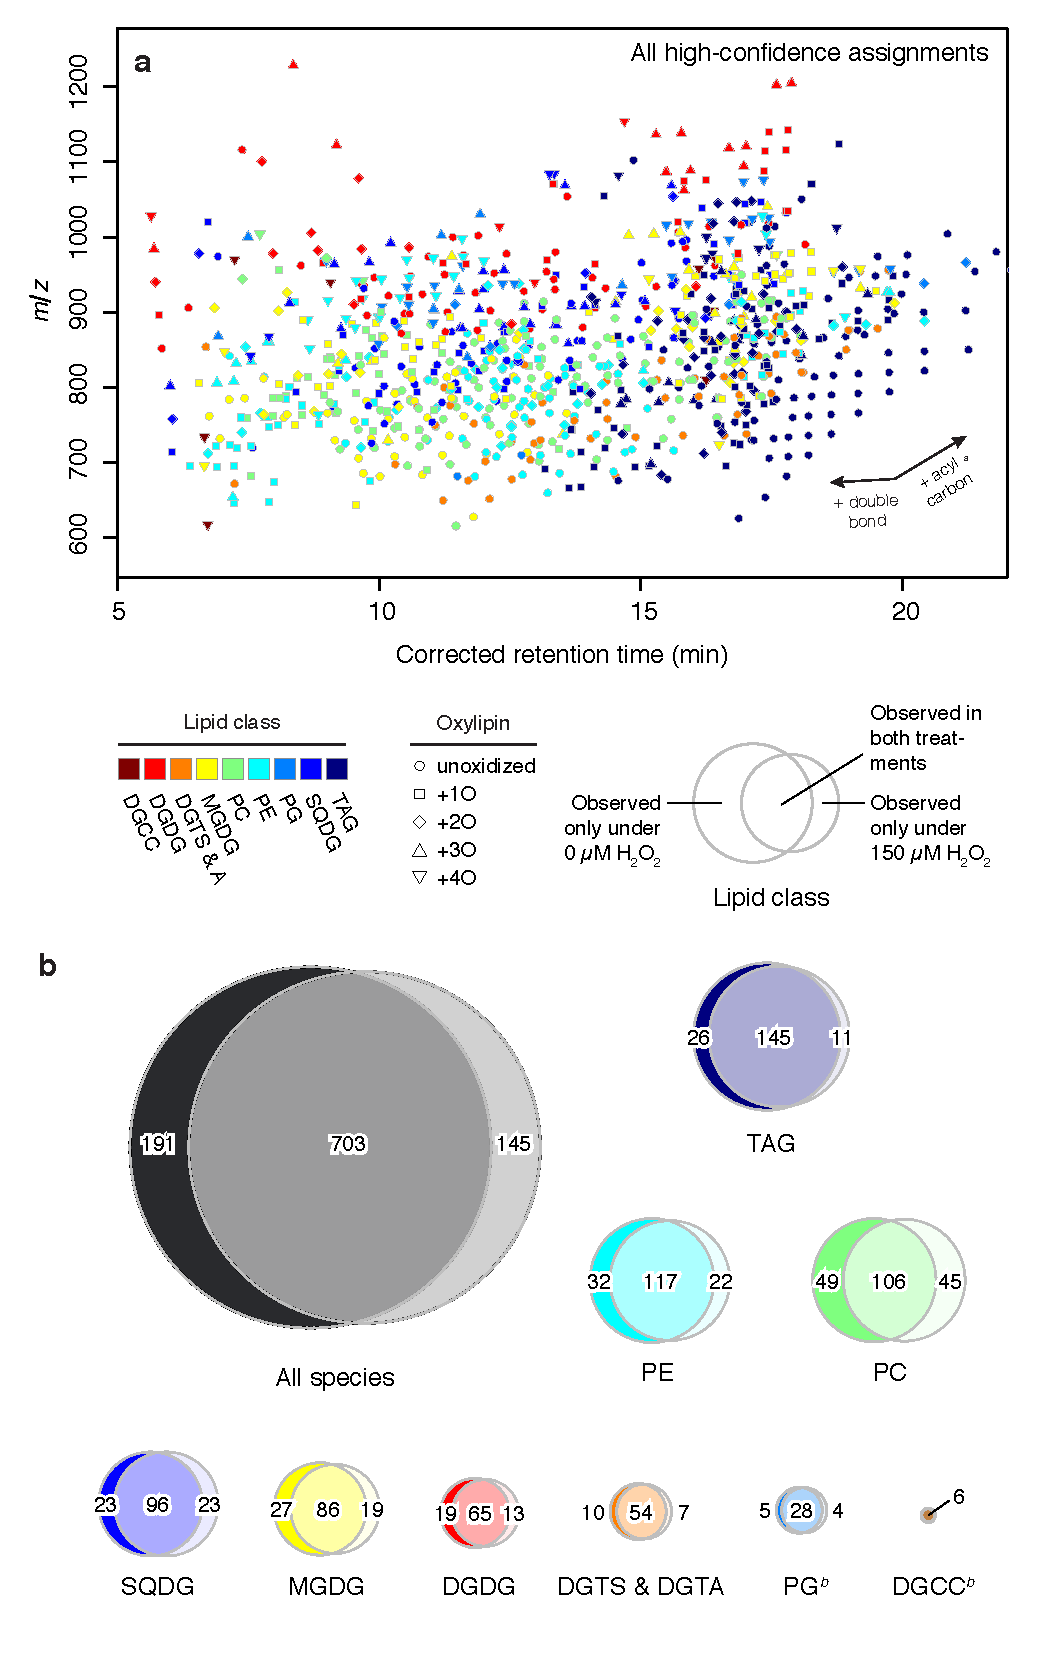
\includegraphics[width=.65\textwidth]{Fig_3-2.pdf}
\captionsetup{font={footnotesize}}
\caption[IPL, ox-IPL, and TAG identified in the \emph{P. tricornutum} dataset]{(a) All IPL, ox-IPL, and TAG identified in the \emph{P. tricornutum} dataset with high confidence (\emph{N} = 1039; figure excludes pigments). (b) Distribution by lipid class of high-confidence assignments made in the 0 and 150 $\mu$M H\textsubscript{2}O\textsubscript{2} treatments at 24 h (\emph{N} = 894 and \emph{N} = 848, respectively). Ellipse size in (b) reflects the number of compounds identified within each class and treatment. The assignments presented in (a) and (b) fully satisfied the LOBSTAHS adduct hierarchy screening criteria (i.e., annotated ``C1'' or ``C2a'' according to the logic in \autoref{fig:c3n1}) and had no competing assignments, such as possible structural isomers, identified in the dataset. Excluded are those compounds having an odd total number of acyl carbon atoms.\\
\emph{\textsuperscript{a}} General direction of movement within \emph{m/z} versus RT plot, for a given lipid class and oxidation state. The direction of movement that results from addition or removal of additional oxygen atom(s) varies by lipid class.\\
\emph{\textsuperscript{b}} Not to scale.}
\label{fig:c3n2}
\end{SCfigure}

The identities of 1,163, or 57\%, of these final database assignments were unique within the scope of our database, meaning the underlying features were matched in the final dataset to only one possible parent compound. 1,149 of these assignments were either IPL, ox-IPL, or TAG (\autoref{fig:c3n2}a); the remainder were photosynthetic pigments. We classified 1,056 of these identifications as ``high confidence,'' indicating that the distribution of adducts present in the constituent features perfectly satisfied the adduct hierarchy rules (\autoref{fig:c3n2}a and symbols with darkest tones in \autoref{fig:adn2}-\autoref{fig:adn10}); these were used in the analysis below.

\subsubsection{Identification and Annotation of Isomers and Isobars}

The remaining 893 assignments (43.4\%) were characterized by some degree of ambiguity, meaning the dataset contained at least one isobar or structural functional isomer of the underlying features (\autoref{table:adn7}; symbols with lightest tones in Figures \autoref{fig:adn2}-\autoref{fig:adn10}). In 752 instances, the dominant adduct of the parent compound was a (functional) structural isomer of the dominant adduct of a different compound assigned from the database (\autoref{table:adn9}, first example). In 195 cases, the dominant adduct ion of the parent compound was an isobar of the primary adduct ion of a different compound (\autoref{table:adn9}, second example). Although these ambiguous assignments represented 43.4\% of all assignments in the screened dataset, they belonged to just 25\% of retained features (27\% of peak groups; \autoref{table:adn7}). The difference was due to the presence of a small number of features (793) whose 54 assignments were doubly ambiguous, i.e., having both isobars and functional structural isomers (symbols with two-tone shading in \autoref{fig:adn2}-\autoref{fig:adn10}; \autoref{table:adn9}, third example). The number of competing assignments for each identified compound varied largely by lipid class. For example, LOBSTAHS found no functional structural isomers for compounds identified in several lipid classes: digalactosyldiacylglycerol (DGDG), phosphatidylethanolamine (PE), and sulfoquinovosyldiacylglycerol (SQDG) (\autoref{fig:adn3}, \autoref{fig:adn7}, and \autoref{fig:adn9}). Doubly ambiguous assignments were confined to only four classes: diacylglyceryl carboxyhydroxymethylcholine (DGCC), diacylglyceryl trimethylhomoserine and diacylglyceryl hydroxymethyl-trimethyl-$\beta$-alanine (DGTS \& DGTA), phosphatidylcholine (PC), and phosphatidylglycerol (PG) (\autoref{fig:adn2}, \autoref{fig:adn4}, \autoref{fig:adn6}, and \autoref{fig:adn8}).

\subsubsection{Annotation of Potential Regioisomers}

LOBSTAHS also identified regioisomers for 352 unique parent compounds in the \emph{P. tricornutum} lipidome (\autoref{table:adn7}; symbols with black dots in \autoref{fig:adn2}-\autoref{fig:adn10}). These were instances in which the same assignment was applied to two or more features appearing at different retention times in the same sample. Many of these assignments were oxylipins and ox-IPL, indicating the presence of multiple oxidized isomers of the same parent IPL that could be used as biomarkers for oxidative stress. Without further analysis, we were unable to determine whether these isomers represented the oxidation of a fatty acid by the same mechanism at a different acyl carbon position, or instead the presence of different oxidized functional groups that yielded equivalent exact masses (e.g., a dihydroxy-, hydroperoxy-, or $\alpha$- or $\gamma$-ketol acid). The level of identification and annotation provided by LOBSTAHS supports a wide range of possible molecular structures for each assignment; an example from the dataset is presented in \autoref{table:adn9}. The data were consistent with studies in both model plant (Buseman et al., 2006; Vu et al., 2012) and animal (Ni et al., 2015) systems that demonstrated the coexistence of a diversity of ox-IPL with both their parent IPL and smaller, traditional oxylipin degradation products.

\subsection{Evaluation of Screening and Identification Performance using Two Methods}

As a means of validating the accuracy and reliability of our approach, we asked LOBSTAHS to identify and annotate all species present in 5 quality control (QC) samples of known composition that were interspersed randomly with samples from the \emph{P. tricornutum} dataset prior to analysis on the mass spectrometer (\autoref{table:c3n1}; \autoref{table:adn6}). The samples contained a mixture of authentic IPL standards that has been used extensively in other work in our laboratory (Popendorf et al., 2013; Van Mooy and Fredricks, 2010). Because the choice of pre-processing software can have a significant impact on feature detection (Cajka and Fiehn, 2016), we conducted parallel analyses with both xcms/CAMERA and an alternative program, MAVEN (Clasquin et al., 2012; Melamud et al., 2010). In both cases, LOBSTAHS correctly identified all components of the standard mixture without ambiguity (\autoref{table:c3n1}; \autoref{table:adn6}). Because purified standards do not exist for long-chain ox-IPL, we were unable to directly evaluate the Type 1 error rate for their identification. As a second means of validation, we compared assignments in the screened dataset to two independent inventories of the \emph{P. tricornutum} lipidome (Abida et al., 2015; Levitan et al., 2015). LOBSTAHS found and identified with high confidence 13 of the 16 most abundant IPL and TAG species in one inventory (Abida et al., 2015), and nearly all those in the other (Levitan et al., 2015). While our approach also correctly identified the three remaining components in the former study (PG 32:1, PG 36, and DGTS \& DGTA 40:10), functional structural isomers or isobars made unambiguous identification impossible without further manual inspection of MS\textsuperscript{2} spectra.

\subsection{Resilience of Core \emph{P. tricornutum} Lipidome under Oxidative Stress}

Evidence of the effect of oxidative stress on the lipidome of \emph{P. tricornutum} was observed through comparison of compounds identified in 0 and 150 $\mu$M H\textsubscript{2}O\textsubscript{2} treatments at 24 h (\autoref{fig:c3n2}, \autoref{fig:c3n3}a,b, and \autoref{table:adn9}). That the two treatments produced only subtle differences in molecular diversity (\autoref{fig:c3n2}b) suggests much of the core lipid inventory remained robust to the imposed oxidative stress. The vast majority of the 949 oxidized and unoxidized lipid moieties we identified in the healthy organism (879, or 92.6\%) could still be identified in the lipidome of the stressed cultures (\autoref{fig:c3n2}b). On the basis of peak area, oxidized lipid moieties accounted for 5-7\% of the \emph{P. tricornutum} lipidome across nearly all treatments and timepoints. Based on the relatively consistent size of this oxidized lipid fraction and its persistence in even the 0 $\mu$M H\textsubscript{2}O\textsubscript{2} treatment, we consider it a quantitative constraint on the baseline level of lipid peroxidation associated with metabolic processes in photosynthetic organisms (Apel and Hirt, 2004; Crastes de Paulet et al., 1988).

\begin{SCfigure}[1][!t]
\centering
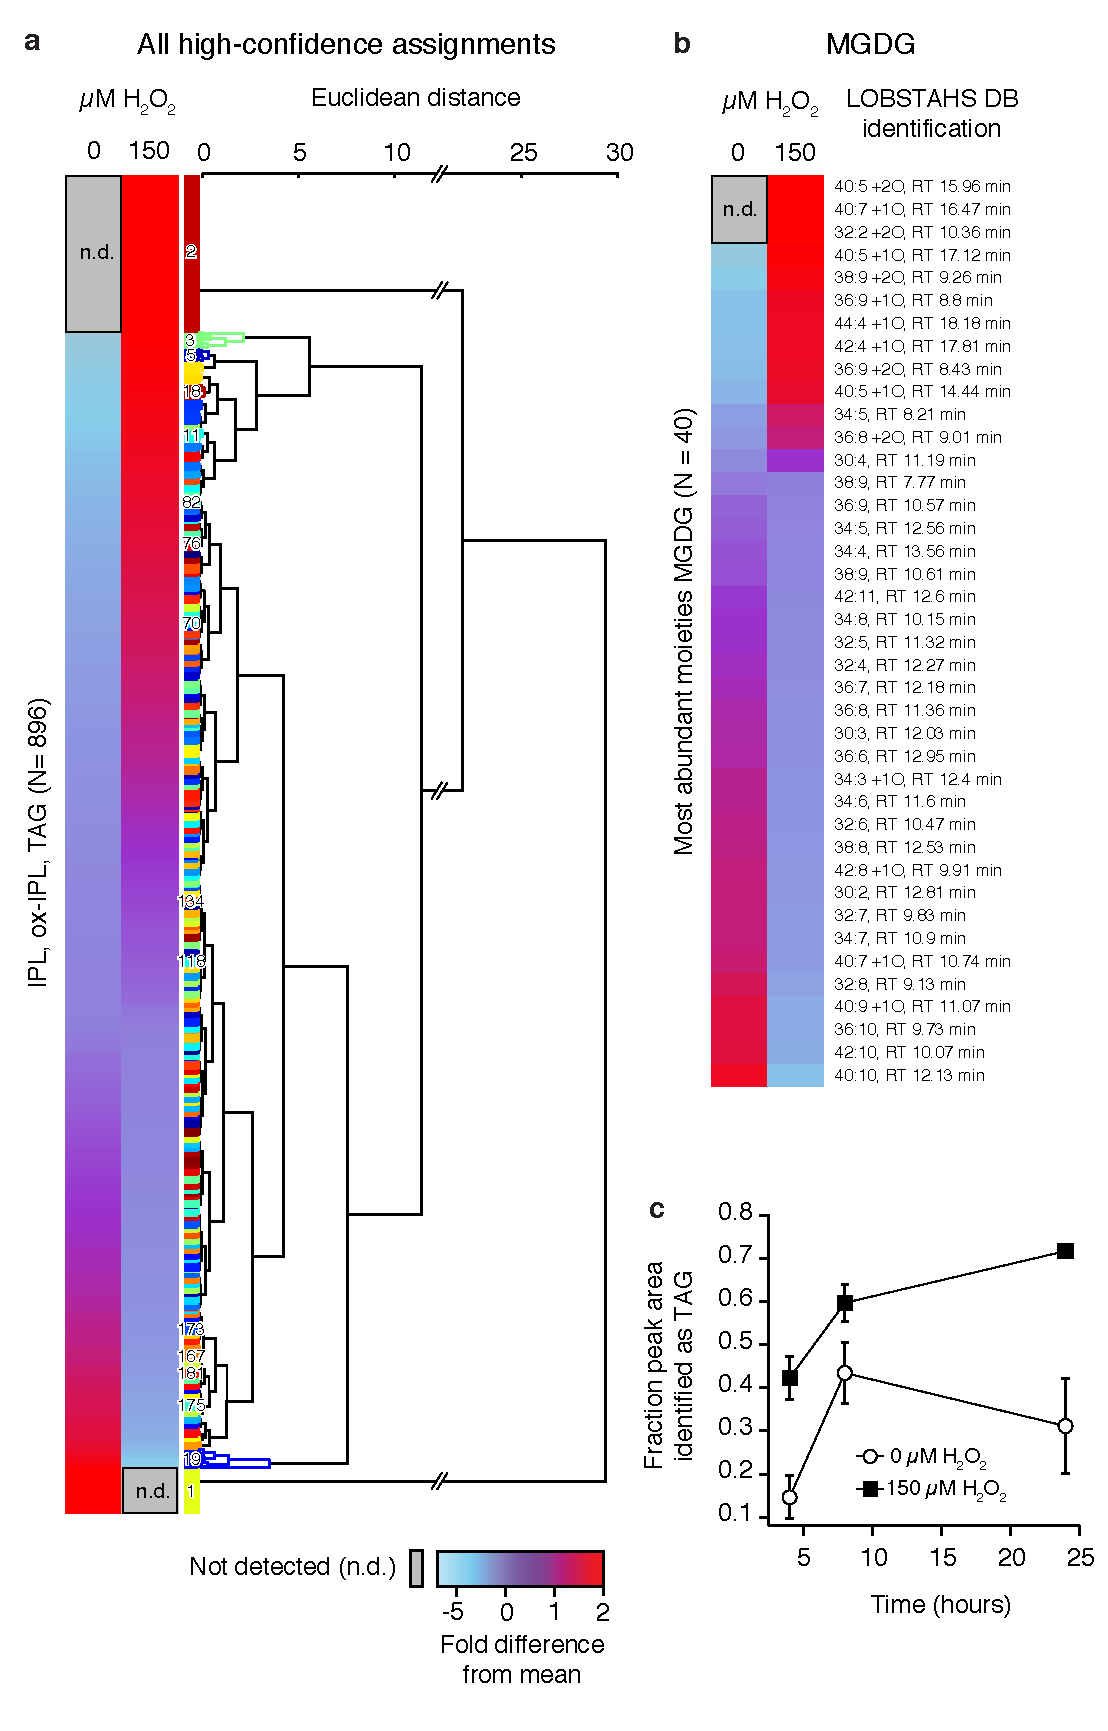
\includegraphics[width=.55\textwidth]{Fig_3-3.pdf}
\captionsetup{font={footnotesize}}
\caption[Remodeling of the \emph{Phaeodactylum tricornutum} lipidome after 24 h, as visualized from data analyzed with LOBSTAHS]{Remodeling of the \emph{Phaeodactylum tricornutum} lipidome after 24 h, as visualized from data analyzed with LOBSTAHS. (a) Heatmap showing relative abundances across two treatments (0 and 150 $\mu$M H\textsubscript{2}O\textsubscript{2}) of all IPL, ox-IPL, and TAG identified with high confidence. Each row (\emph{N} = 896) represents a different compound identified from the database; \autoref{fig:adn11} contains an expanded version of the plot that includes labels for each individual compound. (b) Heatmap detail, showing changes in the most abundant (\emph{N} = 40) moieties of monogalactosyldiacylglycerol (MGDG), a lipid typically localized to the chloroplast. (c) Fraction of total peak area identified as triacylglycerol (TAG) at three timepoints during the experiment. Error bars are $\pm$ SD of two replicates. In (a) and (b), shading shows the relative abundance of each compound as a fold difference of the mean peak area observed in that treatment from the mean peak area of the compound observed across all treatments. Dendrogram clustering and group definitions were determined by similarity profile analysis (Clarke et al., 2008). The numbers and identities of the components assigned to each group in (a) are given in \autoref{table:adn5} and \autoref{fig:adn11}. Solid black lines in the dendrogram indicate branching that was statistically significant (\emph{p} $\leq$ 0.01).}
\label{fig:c3n3}
\end{SCfigure}

\subsection{Differences in Degree of Remodeling Between Lipid Classes and Functional Groupings}

We used similarity profile analysis of the scaled LOBSTAHS data (Clarke et al., 2008) to place the annotated features into 181 groups of components which clustered significantly according to their behavior (\autoref{fig:c3n3} and \autoref{fig:adn1}1). The components of each group are given in \autoref{table:adn8}. We further examined the up- and downregulation of lipidome components under oxidative stress by dividing potential biomarkers into classes based on their molecular headgroups (\autoref{table:adn9}). This allowed us to examine class-specific differences in the number of acyl carbon atoms, acyl carbon-to-carbon double bonds, and oxidation states (i.e., additional oxygen atoms) of component lipids under the two treatments. Differential expression of chemical properties within several classes (\autoref{fig:c3n3}; \autoref{table:adn9}) suggested the \emph{P. tricornutum} lipidome was remodeled in subtle but pervasive ways.

\subsection{Fatty Acid Chain Elongation is an Apparent Response to Oxidative Stress in the Chloroplast}

Oxidative stress appeared to induce elongation of fatty acids throughout the \emph{P. tricornutum} lipidome (\autoref{table:adn9}). Lipid moieties upregulated by oxidative stress had longer fatty acid chains than those that were downregulated. We observed the greatest breadth of structural change in monogalactosyldiacylglycerol (MGDG), a lipid typically localized to the chloroplast (\autoref{table:adn9}; \autoref{fig:c3n3}b). Moieties of MGDG upregulated in the 150 $\mu$M H\textsubscript{2}O\textsubscript{2} treatment had significantly longer fatty acid chains and were more oxidized than those downregulated under oxidative stress; oxidation and elongation were also accompanied by a statistically significant decrease in acyl chain unsaturation (\autoref{table:adn9}). The MGDG moieties responsible for these shifts in class structural properties were confined largely to groups 1, 2, 4, 5, 7, 9, 12, 166, 167, and 180 in our similarity profile analysis (\autoref{fig:c3n3}b and \autoref{fig:adn11}; \autoref{table:adn8}). Lipid oxidation has been previously linked in the diatom \emph{Skeletonema costatum} to lipolytic cleavage of MGDG and phospholipids within the chloroplast, resulting in oxylipin production from free fatty acids (d'Ippolito et al., 2004). While intact oxidized MGDG species have not been previously observed in algae, ox-MGDG have been documented in terrestrial plants upon wounding (Vu et al., 2012). The production of ox-IPL in \emph{Arabidopsis thaliana} may be a means of binding ROS within the cell membrane to limit damage elsewhere (M\`{e}ne-Saffran\'{e} et al., 2009).

\subsection{Fatty Acid Chain Elongation Also Evident in Lipids Localized to Other Cell Compartments}

In addition to observations of fatty acid chain elongation in lipids typical of the chloroplast, significant elongation was also observed in moieties of phosphatidylethanolamine (PE) that were upregulated upon treatment with 150 $\mu$M H\textsubscript{2}O\textsubscript{2}. When lipids typical of the chloroplast (DGDG, SQDG, MGDG, and PG), endoplasmic reticulum (PC, PG, PE), and mitochondrion (PE and PG) were considered separately (Jouhet et al., 2010), we found that lipids with longer chain fatty acids were upregulated in mitochondria but not in the endoplasmic reticulum (\autoref{table:adn9}). While our analysis suggested that oxidative stress in \emph{P. tricornutum} resulted in a global shift toward lipids with longer chain fatty acids, the opposite lipidomic response was observed for \emph{P. tricornutum} under nitrogen stress (Yang et al., 2013). Nitrogen stress resulted in a decrease in both eicosapentaenoic (EPA; 20:5) and docosahexaenoic (DHA; 22:6) acids and a shift toward shorter chain length palmitic (16:0) and palmitoleic (16:1) acids (Yang et al., 2013). We do not view the data we obtained using LOBSTAHS as incompatible with these findings; instead, the result suggests that different sources of stress upon the cell can induce specific and distinct signatures in the lipidome of \emph{P. tricornutum}.

\subsection{Significant Enrichment Observed in TAG}

Whereas the impact of oxidative stress within most lipid classes was confined to relatively modest changes in structural properties, treatment with 150 $\mu$M H\textsubscript{2}O\textsubscript{2} induced a very significant enrichment in the fraction of peak area we identified as triacylglycerols (TAG; \autoref{fig:c3n3}c). Enigmatically, the TAG moieties upregulated in the 150 $\mu$M treatment were significantly less oxidized than those downregulated (\autoref{table:adn9}). We hypothesize that the growth of this chemically reduced TAG pool may be evidence of enhanced \emph{de novo} production of un-oxidized TAG as a response to oxidative stress. Increased TAG synthesis is a known response to nutrient starvation in virtually all algae (Goncalves et al., 2016; Merchant et al., 2012), including in \emph{P. tricornutum} (Abida et al., 2015; Levitan et al., 2015). While increased TAG production in algae has not been previously linked directly to oxidative stress, increased production has been observed as a response to viral infection in the haptophyte alga \emph{Emiliania huxleyi} (Hunter et al., 2015).

\subsection{No Overall Increase Observed in Lipidome Oxidation State}

Enigmatically, we found no statistically significant differences in either the peak area allocated to oxidized lipid moieties or in the fraction of unique compounds identified as oxidized (\autoref{table:adn9}; calculations not shown). One explanation for this finding is that the cultures were not sampled soon enough after treatment with H\textsubscript{2}O\textsubscript{2} to observe oxidation of the lipidome before a rapid antioxidant response was induced in the organism. By 4 hours, the first timepoint at which the experiment was sampled, it is not unreasonable to expect that repair of much of the initial oxidative damage would already have been underway via upregulation of a suite of enzymatic and non-enzymatic plant antioxidant defense mechanisms (Lesser, 2006; Gill and Tuteja, 2010). In \emph{Arabidopsis thaliana}, the lipidomic response to wounding, another source of oxidative stress, was nearly instantaneous; concentrations of several intact oxidized lipid species increased by as much three orders of magnitude within 15 minutes after the treatment was applied (Buseman et al., 2006).

\section{Conclusion}

Using a model dataset, LOBSTAHS allowed us to identify differences in lipid speciation between treatments that could be used as potential indicators oxidative stress in \emph{P. tricornutum}. This potential extended beyond individual oxylipins and ox-IPL to sets of highly interrelated compounds that represented different stages of degradation and oxidation within the same lipidome (\autoref{fig:c3n3} and \autoref{fig:adn11}; \autoref{table:adn8}). While we demonstrated our approach using culture data from a single marine diatom, we designed LOBSTAHS so it can be used with exact-mass HPLC/MS data from virtually any experiment or natural system.

For a minority of features in the screened dataset that had isobars and/or structural isomers (\autoref{table:adn7}; \autoref{fig:adn2}-\autoref{fig:adn10}), we were unable to make unambiguous identifications using LOBSTAHS alone. Many of these could be identified more rigorously through comparison with results from alternative commercial software or by manual inspection using authentic standards or diagnostic MS fragmentation patterns. Our objective, however, was not to definitively characterize a few individual compounds with absolute certainty, but instead to putatively identify a broad range of possible biomarkers for further analysis and discovery with a level of certainty between Level 3 (``Putatively characterized compound classes'') and Level 2 (``Putatively annotated compounds''), using the scheme of Sumner et al. (2007), The overall results we obtained with the \emph{P. tricornutum} dataset demonstrate the ability of LOBSTAHS to assist in this task. The screening and annotation process allowed us to assess a range of levels of confidence on the putative assignments, producing an ample subset of high-confidence compound identifications sufficient to facilitate a detailed statistical analysis. Future integration of methods such as chiral HPLC (Senger et al., 2005) or matching of diagnostic MS\textsuperscript{2} fragmentation spectra, with screening tools such as the one we present here will assist in discovery of biomarkers in larger datasets and with even greater confidence.

\section{Acknowledgments }

We thank Elizabeth Kujawinski, Winn Johnson, and Krista Longnecker for discussions on the analysis of metabolomics datasets and assistance with xcms; Marian Carlson and Matthew Johnson for discussions on the effects of oxidative stress in microorganisms; Assaf Vardi and Daniella Schatz for providing the \emph{P. tricornutum} cell cultures; and Eugene Melamud for answering our many questions about MAVEN. Liz Kujawinski provided thoughtful feedback on an earlier version of the manuscript. Finally, we thank two anonymous reviewers for critical comments that improved the manuscript significantly. This research was supported by the Gordon and Betty Moore Foundation through Grant GBMF3301 to B.A.S.V.M. This research was also funded in part by a grant to B.A.S.V.M. from the Simons Foundation and is a contribution of the Simons Collaboration on Ocean Processes and Ecology (SCOPE). J.R.C. acknowledges support from a U.S. Environmental Protection Agency (EPA) STAR Graduate Fellowship (Fellowship Assistance Agreement no. FP-91744301-0).

\section{Availability of Data and Code }

The current release of the LOBSTAHS package can be compiled using R devtools from source files maintained at \url{https://github.com/vanmooylipidomics/LOBSTAHS}. A readme file and R vignette in the repository contain step-by-step installation and operation instructions. The fully processed \emph{Phaeodactylum tricornutum} dataset is available from \url{https://github.com/vanmooylipidomics/PtH2O2lipids} as the R data package PtH2O2lipids. Both packages are provided under the MIT License. Auxiliary R scripts necessary for pre-processing of data are maintained at \url{https://github.com/vanmooylipidomics/LipidomicsToolbox}. Raw files for the \emph{P. tricornutum} dataset may be downloaded at \url{ftp://ftp.whoi.edu/pub/science/MCG/gbmf/VanMooy/OxylipinAnalysis}; metadata for the dataset are provided at \url{http://www.whoi.edu/page.do?pid=133616\&tid=282\&cid=192529/}. Scripts used for statistical analysis of the \emph{P. tricornutum} dataset and to produce the figures presented in the text are available from \url{https://github.com/jamesrco/LipidomicsDataViz}. See also \autoref{sec:Supplementary Methodological Details Not Described in the Text}.

\clearpage
\begin{singlespace}
\section*{References}
\addtocounter{section}{1}
{\setlength{\parindent}{0pt}
Abida, H., L. J. Dolch, C. Mei, V. Villanova, M. Conte, M. A. Block, G. Finazzi, O. Bastien, L. Tirichine, C. Bowler, F. Rebeille, D. Petroutsos, J. Jouhet and E. Marechal (2015), Membrane glycerolipid remodeling triggered by nitrogen and phosphorus starvation in \emph{Phaeodactylum tricornutum}, \emph{Plant Physiology}, 167(1), 118-36, doi:\href{http://dx.doi.org/10.1104/pp.114.252395}{10.1104/pp.114.252395}.

{\setlength{\parskip}{10pt}

Andreou, A., F. Brodhun and I. Feussner (2009), Biosynthesis of oxylipins in non-mammals, \emph{Progress in Lipid Research}, 48(3-4), 148-170, doi:\href{http://dx.doi.org/10.1016/J.Plipres.2009.02.002}{10.1016/J.Plipres.2009.02.002}.

Andreou, A. and I. Feussner (2009), Lipoxygenases: Structure and reaction mechanism, \emph{Phytochemistry} 70(13-14), 1504-1510, doi:\href{http://dx.doi.org/10.1016/J.Phytochem.2009.05.008}{10.1016/J.Phytochem.2009.05.008}.

Apel, K. and H. Hirt (2004), Reactive oxygen species: Metabolism, oxidative stress, and signal transduction, \emph{Annual Review of Plant Biology}, 55(1), 373-399, doi:\href{http://dx.doi.org/10.1146/annurev.arplant.55.031903.141701}{10.1146/annurev.arpla\\nt.55.031903.141701}.

Balestra, C., L. Alonso-Saez, J. M. Gasol and R. Casotti (2011), Group-specific effects on coastal bacterioplankton of polyunsaturated aldehydes produced by diatoms, \emph{Aquatic Microbial Ecology}, 63(2), 123-131, doi:\href{http://dx.doi.org/10.3354/Ame01486}{10.3354/Ame01486}.

Balvers, M. G., K. C. Verhoeckx, S. Bijlsma, C. M. Rubingh, J. Meijerink, H. M. Wortelboer and R. F. Witkamp (2012), Fish oil and inflammatory status alter the n-3 to n-6 balance of the endocannabinoid and oxylipin metabolomes in mouse plasma and tissues, \emph{Metabolomics} 8(6), 1130-1147, doi:\href{http://dx.doi.org/10.1007/s11306-012-0421-9}{10.1007/s11306-012-0421-9}.

Benton, H. P., E. J. Want and T. M. D. Ebbels (2010), Correction of mass calibration gaps in liquid chromatography-mass spectrometry metabolomics data, \emph{Bioinformatics}, 26(19), 2488-2489.

Bligh, E. G. and W. J. Dyer (1959), A rapid method of total lipid extraction and purification, \emph{Canadian Journal of Biochemistry and Physiology}, 37, 911-917.

Br\"{u}gger, B. (2014), Lipidomics: analysis of the lipid composition of cells and subcellular organelles by electrospray ionization mass spectrometry, \emph{Annual Review of Biochemistry}, 83(1), 79-98, doi:\href{http://dx.doi.org/10.1146/annurev-biochem-060713-035324}{10.1146/annurev-biochem-060713-035324}.

Bruins, M. J., A. D. Dane, K. Strassburg, R. J. Vreeken, J. W. Newman, N. Salem, Jr., C. Tyburczy and J. T. Brenna (2013), Plasma oxylipin profiling identifies polyunsaturated vicinal diols as responsive to arachidonic acid and docosahexaenoic acid intake in growing piglets, \emph{Journal of Lipid Research}, 54(6), 1598-607, doi:\href{http://dx.doi.org/10.1194/jlr.M034918}{10.1194/jlr.M034918}.

Buseman, C. M., P. Tamura, A. A. Sparks, E. J. Baughman, S. Maatta, J. Zhao, M. R. Roth, S. W. Esch, J. Shah, T. D. Williams and R. Welti (2006), Wounding stimulates the accumulation of glycerolipids containing oxophytodienoic acid and dinor-oxophytodienoic acid in Arabidopsis leaves, \emph{Plant Physiology}, 142(1), 28-39, doi:\href{http://dx.doi.org/10.1104/pp.106.082115}{10.1104/pp.106.082115}.

Cajka, T., and O. Fiehn (2016), Toward merging untargeted and targeted methods in mass spectrometry-based metabolomics and lipidomics, \emph{Analytical Chemistry}, 88(1), 524-545, doi:\href{http://dx.doi.org/10.1021/acs.analchem.5b04491}{10.1021/acs.analchem.5b04491}.

Carini, P., B. A. S. Van Mooy, J. C. Thrash, A. White, Y. Zhao, E. O. Campbell, H. F. Fredricks and S. J. Giovannoni (2015), SAR11 lipid renovation in response to phosphate starvation, \emph{Proceedings of the National Academy of Sciences of the United States of America}, 112(25), 7767-7772, doi:\href{http://dx.doi.org/10.1073/pnas.1505034112}{10.1073/pnas.1505034112}.

Casotti, R., S. Mazza, C. Brunet, V. Vantrepotte, A. Ianora and A. Miralto (2005), Growth inhibition and toxicity of the diatom aldehyde 2-trans, 4-trans-decadienal on \emph{Thalassiosira weissflogii} (bacillariophyceae), \emph{Journal of Phycology}, 41(1), 7-20, doi:\href{http://dx.doi.org/10.1111/j.1529-8817.2005.04052.x}{10.1111/j.1529-8817.20\\05.04052.x}.

Clarke, K. R., P. J. Somerfield and R. N. Gorley (2008), Testing of null hypotheses in exploratory community analyses: similarity profiles and biota-environment linkage, \emph{Journal of Experimental Marine Biology and Ecology}, 366(1--2), 56-69, doi:\href{http://dx.doi.org/10.1016/j.jembe.2008.07.009}{10.1016/j.jembe.2008.07.009}.

Clasquin, M. F., E. Melamud and J. D. Rabinowitz (2012), LC-MS data processing with MAVEN: a metabolomic analysis and visualization engine, \emph{Current Protocols in Bioinformatics}, 37, 14.11:14.11.1--14.11.23, doi:\href{http://dx.doi.org/10.1002/0471250953.bi1411s37}{10.1002/0471250953.bi1411s37}.

Crastes de Paulet, A., L. Douste-Blazy and R. Paoletti, eds. (1988), \emph{Free Radicals, Lipoproteins, and Membrane Lipids}, Plenum Publishing Corporation, New York.

d'Ippolito, G., S. Tucci, A. Cutignano, G. Romano, G. Cimino, A. Miralto and A. Fontana (2004), The role of complex lipids in the synthesis of bioactive aldehydes of the marine diatom \emph{Skeletonema costatum}, \emph{Biochimica et Biophysica Acta}, 1686(1-2), 100-107, doi:\href{http://dx.doi.org/10.1016/J.Bblalip.2004.09.002}{10.1016/J.Bbl\\alip.2004.09.002}.

Dooley, C. T., T. M. Dore, G. T. Hanson, W. C. Jackson, S. J. Remington and R. Y. Tsien (2004), Imaging dynamic redox changes in mammalian cells with green fluorescent protein indicators, \emph{Journal of Biological Chemistry}, 279(21), 22284-93, doi:\href{http://dx.doi.org/10.1074/jbc.M312847200}{10.1074/jbc.M312847200}.

Edwards, B. R., K. D. Bidle and B. A. S. Van Mooy (2015), Dose-dependent regulation of microbial activity on sinking particles by polyunsaturated aldehydes: Implications for the carbon cycle, \emph{Proceedings of the National Academy of Sciences of the United States of America}, 112(19), 5909-5914, doi:\href{http://dx.doi.org/10.1073/pnas.1422664112}{10.1073/pnas.1422664112}.

Ejsing, C. S., E. Duchoslav, J. Sampaio, K. Simons, R. Bonner, C. Thiele, K. Ekroos and A. Shevchenko (2006), Automated identification and quantification of glycerophospholipid molecular species by multiple precursor ion scanning, \emph{Analytical Chemistry}, 78(17), 6202-14, doi:\href{http://dx.doi.org/10.1021/ac060545x}{10.1021/ac060545x}.

Fulton, J. M., H. F. Fredricks, K. D. Bidle, A. Vardi, B. J. Kendrick, G. R. DiTullio and B. A. S. Van Mooy (2014), Novel molecular determinants of viral susceptibility and resistance in the lipidome of \emph{Emiliania huxleyi}, \emph{Environmental Microbiology}, 16(4), 1137-1149, doi:\href{http://dx.doi.org/10.1111/1462-2920.12358}{10.1111/1462-2920.12358}.

Gill, S. S., and N. Tuteja (2010), Reactive oxygen species and antioxidant machinery in abiotic stress tolerance in crop plants, \emph{Plant Physiology and Biochemistry}, 48, 909-930.

Girotti, A. W. (1998), Lipid hydroperoxide generation, turnover, and effector action in biological systems, \emph{Journal of Lipid Research}, 39(8), 1529-1542.

Goncalves, E. C., A. C. Wilkie, M. Kirst and B. Rathinasabapathi (2016), Metabolic regulation of triacylglycerol accumulation in the green algae: identification of potential targets for engineering to improve oil yield, \emph{Plant Biotechnology Journal}, 14(8), 1649-60, doi:\href{http://dx.doi.org/10.1111/pbi.12523}{10.1111/pbi.12523}.

Haller, E., G. St\"{u}biger, D. Lafitte, W. Lindner and M. L\"{a}mmerhofer (2014), Chemical recognition of oxidation-specific epitopes in low-density lipoproteins by a nanoparticle based concept for trapping, enrichment, and liquid chromatography-tandem mass spectrometry analysis of oxidative stress biomarkers, \emph{Analytical Chemistry}, 86(19), 9954-9961, doi:\href{http://dx.doi.org/10.1021/ac502855n}{10.1021/ac50\\2855n}.

Hanson, G. T., R. Aggeler, D. Oglesbee, M. Cannon, R. A. Capaldi, R. Y. Tsien and S. J. Remington (2004), Investigating mitochondrial redox potential with redox-sensitive green fluorescent protein indicators, \emph{Journal of Biological Chemistry}, 279(13), 13044-53, doi:\href{http://dx.doi.org/10.1074/jbc.M312846200}{10.1074/jbc.M312846200}.

Hol\v{c}apek, M. (2015), Lipidomics, \emph{Analytical and Bioanalytical Chemistry}, 407(17), 4971-4972, doi:\href{http://dx.doi.org/10.1007/s00216-015-8740-0}{10.1007/s00216-015-8740-0}.

Hummel, J., S. Segu, Y. Li, S. Irgang, J. Jueppner and P. Giavalisco (2011), Ultra performance liquid chromatography and high resolution mass spectrometry for the analysis of plant lipids, \emph{Frontiers in Plant Science}, 2, 54, doi:\href{http://dx.doi.org/10.3389/Fpls.2011.00054}{10.3389/Fpls.2011.00054}.

Hunter, J. E., M. J. Frada, H. F. Fredricks, A. Vardi and B. A. S. Van Mooy (2015), Targeted and untargeted lipidomics of \emph{Emiliania huxleyi} viral infection and life cycle phases highlights molecular biomarkers of infection, susceptibility, and ploidy, \emph{Frontiers in Marine Science}, 2, 81, doi:\href{http://dx.doi.org/10.3389/fmars.2015.00081}{10.3389/fmars.2015.00081}.

Husen, P., K. Tarasov, M. Katafiasz, E. Sokol, J. Vogt, J. Baumgart, R. Nitsch, K. Ekroos and C. S. Ejsing (2013), Analysis of lipid experiments (ALEX): a software framework for analysis of high-resolution shotgun lipidomics data, \emph{PLoS One}, 8(11), e79736, doi:\href{http://dx.doi.org/10.1371/journal.pone.0079736}{10.1371/jo\\urnal.pone.0079736}.

Ianora, A. and A. Miralto (2010), Toxigenic effects of diatoms on grazers, phytoplankton and other microbes: a review, \emph{Ecotoxicology}, 19(3), 493-511, doi:\href{http://dx.doi.org/10.1007/S10646-009-0434-Y}{10.1007/S10646-009-0434-Y}.

Kessner, D., M. Chambers, R. Burke, D. Agus, and P. Mallick (2008), ProteoWizard: open source software for rapid proteomics tools development, \emph{Bioinformatics}, 24, 2534-2536.

Kind, T. and O. Fiehn (2006), Metabolomic database annotations via query of elemental compositions: mass accuracy is insufficient even at less than 1 ppm, \emph{BMC Bioinformatics}, 7, 234, doi:\href{http://dx.doi.org/10.1186/1471-2105-7-234}{10.1186/1471-2105-7-234}.

Kuhl, C., R. Tautenhahn, C. Bottcher, T. R. Larson and S. Neumann (2012), CAMERA: an integrated strategy for compound spectra extraction and annotation of liquid chromatography/mass spectrometry data sets, \emph{Analytical Chemistry}, 84(1), 283-9, doi:\href{http://dx.doi.org/10.1021/ac202450g}{10.1021/ac202450g}.

Kuhn, H. and S. Borngraber (1999), Mammalian 15-lipoxygenases: Enzymatic properties and biological implications, in \emph{Lipoxygenases and Their Metabolites}, edited by S. Nigam and C. R. Pace-Asciak, pp. 5-28, Plenum Publishers, New York.

Jouhet, J., E. Dubots, E. Mar\'{e}chal, and M. Block (2010), Lipid trafficking in plant photosynthetic cells, in \emph{Lipids in Photosynthesis}, edited by H. Wada and N. Murata, pp. 349-372, Springer Netherlands, Dordrecht, The Netherlands.

Lamari, N., M. V. Ruggiero, G. d'Ippolito, W. H. C. F. Kooistra, A. Fontana and M. Montresor (2013), Specificity of lipoxygenase pathways supports species delineation in the marine diatom genus \emph{Pseudo-nitzschia}, \emph{PLoS One,} 8(8), e73281, doi:\href{http://dx.doi.org/10.1371/journal.pone.0073281}{10.1371/journal.pone.0073281}.

Layre, E., L. Sweet, S. Hong, C. A. Madigan, D. Desjardins, D. C. Young, T. Y. Cheng, J. W. Annand, K. Kim, I. C. Shamputa, M. J. McConnell, C. A. Debono, S. M. Behar, A. J. Minnaard, M. Murray, C. E. Barry, 3rd, I. Matsunaga and D. B. Moody (2011), A comparative lipidomics platform for chemotaxonomic analysis of \emph{Mycobacterium tuberculosis}, \emph{Chemistry \& Biology,} 18(12), 1537-49, doi:\href{http://dx.doi.org/10.1016/j.chembiol.2011.10.013}{10.1016/j.chembiol.2011.10.013}.

Lesser, M. P. (2006), Oxidative stress in marine environments: biochemistry and physiological ecology, \emph{Annual Review of Physiology}, 68, 253-278.

Levitan, O., J. Dinamarca, E. Zelzion, D. S. Lun, L. T. Guerra, M. K. Kim, J. Kim, B. A. S. Van Mooy, D. Bhattacharya and P. G. Falkowski (2015), Remodeling of intermediate metabolism in the diatom \emph{Phaeodactylum tricornutum }under nitrogen stress, \emph{Proceedings of the National Academy of Sciences of the United States of America}, 112(2), 412-417, doi:\href{http://dx.doi.org/10.1073/pnas.1419818112}{10.1073/pnas.1419818112}.

Libiseller, G., M. Dvorzak, U. Kleb, E. Gander, T. Eisenberg, F. Madeo, S. Neumann, G. Trausinger, F. Sinner, T. Pieber and C. Magnes (2015), IPO: a tool for automated optimization of XCMS parameters, \emph{BMC Bioinformatics}, 16, 118, doi:\href{http://dx.doi.org/10.1186/s12859-015-0562-8}{10.1186/s12859-015-0562-8}.

Melamud, E., L. Vastag and J. D. Rabinowitz (2010) Metabolomic Analysis and Visualization Engine for LC-MS data, \emph{Analytical Chemistry}, 82(23), 9818-9826, doi:\href{http://dx.doi.org/10.1021/ac1021166}{10.1021/ac1021166}.

M\`{e}ne-Saffran\'{e}, L., L. Dubugnon, A. Chetelat, S. Stolz, C. Gouhier-Darimont and E. E. Farmer (2009), Nonenzymatic oxidation of trienoic fatty acids contributes to reactive oxygen species management in \emph{Arabidopsis}, \emph{Journal of Biological Chemistry}, 284(3), 1702-8, doi:\href{http://dx.doi.org/10.1074/jbc.M807114200}{10.1074/jbc.M807114200}.

Merchant, S. S., J. Kropat, B. Liu, J. Shaw and J. Warakanont (2012), TAG, You're it! \emph{Chlamydomonas} as a reference organism for understanding algal triacylglycerol accumulation, \emph{Current Opinion in Biotechnology}, 23(3), 352-363, doi:\href{http://dx.doi.org/10.1016/j.copbio.2011.12.001}{10.1016/j.copbio.2011.12.001}.

Miralto, A., G. Barone, G. Romano, S. A. Poulet, A. Ianora, G. L. Russo, I. Buttino, G. Mazzarella, M. Laabir, M. Cabrini and M. G. Giacobbe (1999), The insidious effect of diatoms on copepod reproduction, \emph{Nature} 402(6758), 173-176.

Ni, Z., I. Milic and M. Fedorova (2015), Identification of carbonylated lipids from different phospholipid classes by shotgun and LC-MS lipidomics, \emph{Analytical and Bioanalytical Chemistry}, 407(17), 5161-5173, doi:\href{http://dx.doi.org/10.1007/s00216-015-8536-2}{10.1007/s00216-015-8536-2}.

Pearson, A. (2014), Lipidomics for geochemistry, in \emph{Treatise on Geochemistry}, vol. 12, edited by H. D. Holland and K. K. Turekian, 2nd ed., pp. 291-336, Elsevier, Oxford.

Pohnert, G. (2008), Influence of algal secondary metabolites on plankton community structure, in \emph{Algal Chemical Ecology}, edited by C. D. Amsler, pp. 195-202, Springer-Verlag, Berlin.

Popendorf, K. J., H. F. Fredricks and B. A. S. Van Mooy (2013), Molecular ion-independent quantification of polar glycerolipid classes in marine plankton using triple quadrupole MS, \emph{Lipids} 48(2), 185-195, doi:\href{http://dx.doi.org/10.1007/s11745-012-3748-0}{10.1007/s11745-012-3748-0}.

R Core Team (2015), R: a language and environment for statistical computing, R Foundation for Statistical Computing, Vienna, Austria.

Ribalet, F., L. Intertaglia, P. Lebaron and R. Casotti (2008), Differential effect of three polyunsaturated aldehydes on marine bacterial isolates, \emph{Aquatic Toxicology}, 86(2), 249-255, doi:\href{http://dx.doi.org/10.1016/J.Aquatox.2007.11.005}{10.1016/J.Aquatox.2007.11.005}.

Rosenwasser, S., S. Graff van Creveld, D. Schatz, S. Malitsky, O. Tzfadia, A. Aharoni, Y. Levin, A. Gabashvili, E. Feldmesser and A. Vardi (2014), Mapping the diatom redox-sensitive proteome provides insight into response to nitrogen stress in the marine environment. \emph{Proceedings of the National Academy of Sciences of the United States of America}, 111(7), 2740-2745, doi:\href{http://dx.doi.org/10.1073/pnas.1319773111}{10.1073/pnas.1319773111}.

Senger, T., T. Wichard, S. Kunze, C. Gobel, J. Lerchl, G. Pohnert and I. Feussner (2005), A multifunctional lipoxygenase with fatty acid hydroperoxide cleaving activity from the moss \emph{Physcomitrella patens}, \emph{Journal of Biological Chemistry,} 280(9), 7588-7596, doi:\href{http://dx.doi.org/10.1074/jbc.M411738200}{10.1074/jbc.M\\411738200}.

Smith, C. A., E. J. Want, G. O'Maille, R. Abagyan and G. Siuzdak (2006), XCMS: processing mass spectrometry data for metabolite profiling using nonlinear peak alignment, matching, and identification, \emph{Analytical Chemistry}, 78, 779-787.

Sparvero, L. J., A. A. Amoscato, P. M. Kochanek, B. R. Pitt, V. E. Kagan and H. Bayır (2010), Mass-spectrometry based oxidative lipidomics and lipid imaging: applications in traumatic brain injury, \emph{Journal of Neurochemistry}, 115(6), 1322-1336, doi:\href{http://dx.doi.org/10.1111/j.1471-4159.2010.07055.x}{10.1111/j.1471-4159.2010.07055.x}.

Spickett, C. M. and A. R. Pitt (2015), Oxidative lipidomics coming of age: advances in analysis of oxidized phospholipids in physiology and pathology, \emph{Antioxidants \& Redox Signaling}, 22(18), 1646-1666, doi:\href{http://dx.doi.org/10.1089/ars.2014.6098}{10.1089/ars.2014.6098}.

Strassburg, K., A. M. Huijbrechts, K. A. Kortekaas, J. H. Lindeman, T. L. Pedersen, A. Dane, R. Berger, A. Brenkman, T. Hankemeier, J. van Duynhoven, E. Kalkhoven, J. W. Newman and R. J. Vreeken (2012), Quantitative profiling of oxylipins through comprehensive LC-MS/MS analysis: application in cardiac surgery, \emph{Analytical and Bioanalytical Chemistry}, 404(5): 1413-26, doi:\href{http://dx.doi.org/10.1007/s00216-012-6226-x}{10.1007/s00216-012-6226-x}.

Sumner, L., A. Amberg, D. Barrett, M. Beale, R. Beger and C. Daykin (2007), Proposed minimum reporting standards for chemical analysis, \emph{Metabolomics}, 3, 211--221.

Tautenhahn, R., C. Boettcher and S. Neumann (2008), Highly sensitive feature detection for high resolution LC/MS, \emph{BMC Bioinformatics} 9, 504.

Thomas, A., N. H. Patterson, M. M. Marcinkiewicz, A. Lazaris, P. Metrakos and P. Chaurand (2013), Histology-driven data mining of lipid signatures from multiple imaging mass spectrometry analyses: application to human colorectal cancer liver metastasis biopsies, \emph{Analytical Chemistry}, 85(5), 2860-2866, doi:\href{http://dx.doi.org/10.1021/ac3034294}{10.1021/ac3034294}.

Triantaphylides, C., M. Krischke, F. A. Hoeberichts, B. Ksas, G. Gresser, M. Havaux, F. Van Breusegem and M. J. Mueller (2008), Singlet oxygen is the major reactive oxygen species involved in photooxidative damage to plants, \emph{Plant Physiology}, 148(2), 960-968, doi:\href{http://dx.doi.org/10.1104/Pp.108.125690}{10.1104/Pp.108.125690}.

van Creveld, S. G., S. Rosenwasser, D. Schatz, I. Koren and A. Vardi (2015), Early perturbation in mitochondria redox homeostasis in response to environmental stress predicts cell fate in diatoms, \emph{ISME Journal}, 9(2), 385-395, doi:\href{http://dx.doi.org/10.1038/ismej.2014.136}{10.1038/ismej.2014.136}.

Van Mooy, B. A. S. and H. F. Fredricks (2010), Bacterial and eukaryotic intact polar lipids in the eastern subtropical South Pacific: Water-column distribution, planktonic sources, and fatty acid composition, \emph{Geochimica et Cosmochimica Acta}, 74(22), 6499-6516, doi:\href{http://dx.doi.org/10.1016/j.gca.2010.08.026}{10.1016/j.\\gca.2010.08.026}.

Van Mooy, B. A. S., H. F. Fredricks, B. E. Pedler, S. T. Dyhrman, D. M. Karl, M. Koblizek, M. W. Lomas, T. J. Mincer, L. R. Moore, T. Moutin, M. S. Rappe and E. A. Webb (2009), Phytoplankton in the ocean use non-phosphorus lipids in response to phosphorus scarcity, \emph{Nature}, 458(7234), 69-72.

Vardi, A. (2008), Cell signaling in marine diatoms, \emph{Communicative \& Integrative Biology}, 1(2), 134-6.

Vardi, A., B. A. S. Van Mooy, H. F. Fredricks, K. J. Popendorf, J. E. Ossolinski, L. Haramaty and K. D. Bidle (2009), Viral glycosphingolipids induce lytic infection and cell death in marine phytoplankton, \emph{Science}, 326(5954), 861-865, doi:\href{http://dx.doi.org/10.1126/science.1177322}{10.1126/science.1177322}.

Vu, H. S., P. Tamura, N. A. Galeva, R. Chaturvedi, M. R. Roth, T. D. Williams, X. Wang, J. Shah and R. Welti (2012), Direct infusion mass spectrometry of oxylipin-containing Arabidopsis membrane lipids reveals varied patterns in different stress responses, \emph{Plant Physiology}, 158(1), 324-339, doi:\href{http://dx.doi.org/10.1104/pp.111.190280}{10.1104/pp.111.190280}.

Wenk, M. R. (2010), Lipidomics: new tools and applications, \emph{Cell}, 143(6), 888-895, doi:\href{http://dx.doi.org/10.1016/j.cell.2010.11.033}{10.101\\6/j.cell.2010.11.033}.

Yang, Z.-K., Y.-F. Niu, Y.-H. Ma, J. Xue, M.-H. Zhang, W.-D. Yang, J.-S. Liu, S.-H. Lu, Y. Guan, and H.-Y. Li (2013), Molecular and cellular mechanisms of neutral lipid accumulation in diatom following nitrogen deprivation, \emph{Biotechnology for Biofuels}, 6, 67.}}
\end{singlespace}

\clearpage

\begin{landscape}
\begin{footnotesize}
\begin{singlespace}
%\renewcommand*{\arraystretch}{1.3}
\begin{longtable}{ Lp{.08\linewidth} Lp{.07\linewidth} Lp{.07\linewidth} Lp{.08\linewidth} Lp{.08\linewidth} Lp{.08\linewidth} Lp{.08\linewidth} Lp{.08\linewidth} Lp{.11\linewidth} Lp{.1\linewidth} }
\captionsetup{font={normalsize}}
\caption[Evaluation of Lipidomics Method Performance using IPL Standards]{Evaluation of Lipidomics Method Performance using IPL Standards}
\label{table:c3n1}
\endfirsthead
\endhead
\toprule
Lipid Class & Origin of Standard & Moieties Present in Standard\emph{\textsuperscript{a}} & Dominant Positive Mode Adduct Ion & Ion Exact \emph{m/z} & Observed \emph{m/z}\emph{\textsuperscript{b}} & Rel. Mass Uncertainty (ppm)\emph{\textsuperscript{c}} & Correct LOBSTAHS ID? & Confidence in Assignment After Adduct Hierarchy Screening\emph{\textsuperscript{d}} & Structural Isomers or Isobars Present After Screening? \\
\midrule
MGDG & Natural & 34:0 & {[}M+NH\textsubscript{4}{]}\textsuperscript{+} & 776.6246 & 776.6248 & 0.2 & Yes & High & No \\

 &  & 36:0& {[}M+NH\textsubscript{4}{]}\textsuperscript{+} & 804.6559 & 804.6561 & 0.3 & Yes & High & No \\

DNP-PE & Synthetic & 32:0 & {[}M+NH\textsubscript{4}{]}\textsuperscript{+} & 875.5505 & 875.5507 & 0.2 & Yes & High & No \\

SQDG & Natural & 34:3 & {[}M+NH\textsubscript{4}{]}\textsuperscript{+} & 834.5396 & 834.5398 & 0.2 & Yes & High & No \\

 &  & 34:2 & {[}M+NH\textsubscript{4}{]}\textsuperscript{+} & 836.5552 & 836.5554 & 0.2 & Yes & High & No \\

PG & Synthetic & 32:0 & {[}M+NH\textsubscript{4}{]}\textsuperscript{+} & 740.5436 & 740.5438 & 0.3 & Yes & High & No \\

PE & Synthetic & 32:0 & {[}M+H{]}\textsuperscript{+} & 692.5225 & 692.5227 & 0.3 & Yes & High & No \\

PC & Synthetic & 32:0 & {[}M+H{]}\textsuperscript{+} & 734.5694 & 734.5696 & 0.2 & Yes & High & No \\

DGDG & Natural & 34:2 & {[}M+NH\textsubscript{4}{]}\textsuperscript{+} & 934.6462 & 934.6463 & 0.1 & Yes & High & Yes \\

 &  & 36:4 & {[}M+NH\textsubscript{4}{]}\textsuperscript{+} & 958.6462 & 958.6463 & 0.1 & Yes & High & Yes \\

Mean &  &  &  &  &  & 0.2 &  &  & \\
\bottomrule
\captionsetup{font={footnotesize}}
\caption*{\emph{\textsuperscript{a}} Multiple moieties were present in glycolipid standards purified from natural samples; only predominant moieties are shown\\
\emph{\textsuperscript{b}} Mean observed \emph{m/z} ratio in 5 independent samples\\
\emph{\textsuperscript{c}} $\left| {\frac{{{\text{Observed exact mass}} - {\text{Database exact mass}}}}{{{\text{Database exact mass}}}}} \right| \times {10^6}$\\
\emph{\textsuperscript{d}} ``High confidence'': Assignment fully satisfied all adduct hierarchy rules and other screening criteria.
}
\end{longtable}
\end{singlespace}
\end{footnotesize}
\end{landscape}

\clearpage

\begin{singlespace}
%\renewcommand*{\arraystretch}{1.3}
\begin{longtable}{ Lp{.02\linewidth} Lp{.39\linewidth} Lp{.11\linewidth} Lp{.11\linewidth} Lp{.11\linewidth} Lp{.11\linewidth} }
\captionsetup{font={normalsize}}
\caption[Progressive Screening and Annotation of the \emph{P. tricornutum} Dataset using xcms, CAMERA, and LOBSTAHS]{Progressive Screening and Annotation of the \emph{P. tricornutum} Dataset using xcms, CAMERA, and LOBSTAHS}
\label{table:c3n2}
\endfirsthead
\endhead
\toprule
 &  & \multicolumn{4}{ l }{No. Present in Dataset} \\
\cmidrule{3-6}
\multicolumn{2}{ l }{Operation(s) Applied} & Peaks & Peak Groups & Database Assign-ments\emph{\textsuperscript{a}}& Unique Parent Compounds \\
\midrule	
\multicolumn{2}{ l }{xcms and CAMERA} &  &  &  \\

 &  &  &  &  &  \\

 & Initial feature detection; pre-processing & 340,991 & 18,314 & --- & --- \\

 &  &  &  &  &  \\

\multicolumn{2}{ l }{LOBSTAHS} &  &  &  &  \\

 &  &  &  &  &   \\

 & Eliminate secondary isotope peaks & 163,938 & 12,146 & --- & --- \\

 &  &  &  &  &  \\

 & Apply initial compound assignments from database & 67,862 & 5,077 & 15,929 & 14,076 \\

 &  &  &  &  &  \\

 & Apply RT screening criteria & 60,070 & 4,451 & 13,504 & 11,779 \\

 &  &  &  &  &  \\

 & Exclude IP-DAG/ TAG with odd total no. of acyl C atoms & 52,337 & 3,871 & 7,458 & 6,283 \\

 &  &  &  &  &  \\

 & Adduct ion hierarchy screening & 21,869 & 1,595 & 2,056\emph{\textsuperscript{b}} & 1,969 \\
\bottomrule
\captionsetup{font={footnotesize}}
\caption*{\emph{\textsuperscript{a}} Figure reflects all assignments from database, including photosynthetic pigments.\\
\emph{\textsuperscript{b}} 1,163, or 57\%, of these had no competing assignments such as functional structural isomers or isobars; these 1,163 assignments represented 990 unique parent compounds.
}
\end{longtable}
\end{singlespace}
